\section{Experimental Setup \& Re-implementation}
\label{sec:reimplement}
This section details the experimental setup used both in the original paper \cite{10.1007/978-3-030-15986-3_19} as well as this paper. It also documents the process of and difficulties during the data collection and evaluation. Lastly, it describes the origins of the datasets used.

\subsection{Experimental Setup}
\citeauthor{10.1007/978-3-030-15986-3_19} used the following tools: (1) Firefox 61.0.2 with Selenium 3.14.0 and geckodriver 0.21.0, (2) Firefox 62.0.2 with Marionette, and (3) Chrome 69 with Chrome DevTools. This multitude of tools was used in order to provide data for a comparison of different frameworks as well as web pages. All pages were loaded on a Thinkpad L450 running Debian 9 (Stretch). The extension used to export HAR files was har-export-trigger 0.6.1. The Thinkpad (i.e. vantage point) was connected directly to a university network to avoid bandwidth / latency issues. To minimize the effects of DNS caching and resolver delay, a recursive resolver within close range (in terms of the network) was used. 

The hardware and software employed in this paper were similar yet more modern. Ubuntu 20.04. was run in a virtual machine on a Matebook X Pro (1st Generation). The use of the following tools was attempted / responsible for the results: (1) Firefox 82 with Selenium 3.141.59 and geckodriver 0.29.0, (2) Firefox 82 with Marionette, and (3) Chrome 88 with Chrome DevTools. The extension used to export HAR files was, as in the original version, har-export-trigger 0.6.1. as no new versions were released since the original paper. The vantage point was connected directly to a stable home network using ethernet; the connection was not shared for the duration of the tests. A recursive DNS resolver close to the vantage point, in terms of the network, was used as well. During testing of scripts in the new environment, there were difficulties; a second virtual machine with the original experimental setup (Debian Stretch, etc.) was used to reproduce / solve these issues. Despite trying the versions specified in the original paper as well as the more modern versions, it was not possible to consistently extract HAR files using Firefox with Selenium and Chrome with PyDevTools as specified in the original paper. 

\subsection{Scripts}
\label{sec:scripts}
All scripts used in \cite{10.1007/978-3-030-15986-3_19} are available in \cite{enghardt_2019}. The scripts are grouped into three categories: measurement / load, computation, and evaluation. The measurement scripts include separate scripts for each of the aforementioned tools (e.g. Firefox with Selenium) as well as a script to parse the exported data and capture packets for comparison with and verification of the results. The computation scripts take the raw results as input and output standardized data that is then used by the evaluation scripts to provide percentiles, averages, and graphs.

The scripts for Firefox with Selenium and Chrome with DevTools were unable to export HAR files in both the Ubuntu virtual machine with all updates installed or a Debian virtual machine using the software versions specified in the original paper. The inability to export the HAR files that were key to the measurements which compared tools led to the decision to focus on reproducing measurements using Firefox with Marionette; this decision meant that results for Chrome could not be reproduced. Multiple of the computation and evaluation scripts also exhibited a number of smaller errors, e.g. the compute script was not compatible with the original data format. The adjusted / corrected scripts are available in a GitHub repository\footnote{\url{https://github.com/curtp67/web-measurement-tools-reproduction}}.
\begin{figure}
		\centering
\begin{subfigure}{\linewidth}
		\includegraphics[width=\linewidth]{New_Plots/ecdf_diff_objectsizes.pdf}
	\caption{New Measurements}
	\label{fig:new_absolute_byte_index}
\end{subfigure}\par\medskip
 \begin{subfigure}{\linewidth}
		\centering
		\includegraphics[width=\linewidth]{Firefox Plots/ecdf_diff_objectsizes.pdf}
	\caption{Original Measurements (Firefox Only)}
	\label{fig:orig_absolute_byte_index}
\end{subfigure}
 \begin{subfigure}{\linewidth}
		\includegraphics[width=\linewidth]{Chrome_Plots/ecdf_diff_objectsizes.pdf}
	\caption{Original Measurements (Chrome Only)}
	\label{fig:orig_chrome_absolute_byte_index}
\end{subfigure}
\caption{Object sizes: differences due to metric for all objects}
	\label{fig:absolute_byte_index}
\end{figure}

\subsection{Datasets}
Alexa Top Lists are, despite some well-known limitations, among the most used data sources for research regarding the internet \cite{10.1145/3278532.3278574}. For this reason, \citeauthor{10.1007/978-3-030-15986-3_19}  used two distinct website lists in their paper: Alexa 1000 (September 18, 2018) and Alexa 10001-11000 (September 30, 2018). Each page was accessed a total of 10 times using different framework over a period of several days. In this paper, I used Alexa 1000 (January 18, 2021) and performed 3 measurements for each website over a period of several days. The original\footnote{\url{http://dx.doi.org/10.14279/depositonce-8100}} and reproduced\footnote{\url{https://syncandshare.lrz.de/getlink/fiFSuxPcpDVkZhwfeTVNDYxc}} datasets collected can be found online. The captured packets (pcap format) that were used to verify results were also not available in the original dataset due to their size; it was, therefore, not possible to compare the original data to them as a baseline for sizes of unencrypted objects, as was done in the original paper. 